\section{Face Recognition with OpenCV2 C++ API: libfacerec}

The C++ API of OpenCV2 closely resembles the \ifx\python\undefined \href{http://www.gnu.org/software/octave/}{GNU Octave}/\href{http://www.mathworks.com}{MATLAB} \else \href{http://www.python.org}{Python} \fi code we've written in section \ref{ssection:example_eigenfaces} and \ref{ssection:example_fisherfaces}. If you have prototyped it with Python or GNU Octave/MATLAB, you won't have a great problem translating it to OpenCV2. I personally think you don't need a book to learn about the OpenCV2 C++ API. There's a lot of documentation coming with OpenCV, just have a look into the \lstinline|doc| folder of your OpenCV installation. The easiest way to get started is the \textit{OpenCV Cheat Sheet (C++)} (\lstinline|opencv_cheatsheet.pdf|), because it shows you how to use all the functions with examples. The \textit{The OpenCV Reference Manual} (\lstinline|opencv2refman.pdf|) is the definite guide to the API (500+ pages). Of course, you'll need a book or other literature for understanding computer vision algorithms - I can't give an introduction to this here.

\subsection{Downloading and Building the libfacerec}

libfacerec is a modern face recognition library for the OpenCV C++ API (BSD license). It has no additional dependencies and implements the Eigenfaces method \cite{PT91}, Fisherfaces method \cite{belhumeru97} and Local Binary Patterns Histograms \cite{Ahonen04}. 

The latest revision of the libfacerec is available at:

\begin{itemize}
   \item \url{https://github.com/bytefish/libfacerec}
\end{itemize}

The library was written for OpenCV 2.3.1 with the upcoming OpenCV 2.4 in mind, so I don't support OpenCV versions earlier than 2.3.1. This project comes as a CMake project with a well-documented API, there's also a tutorial on gender classification. You can see a HTML version of the documentation at:

\begin{itemize}
 \item \url{http://www.bytefish.de/dev/libfacerec/}
\end{itemize}

You can obtain the code by either cloning the repository:

\begin{lstlisting}
git clone git@github.com:bytefish/libfacerec.git
\end{lstlisting}

Or if you don't have \href{http://git-scm.com/}{git} on your system you can download libfacerec as zip or tarball:

\begin{itemize}
	\item \textbf{zip} \url{https://github.com/bytefish/libfacerec/zipball/master}
	\item \textbf{tar} \url{https://github.com/bytefish/libfacerec/tarball/master}
\end{itemize}

Building the demo executables is then as simple as (assuming you are in the top-level directory):

\begin{lstlisting}
mkdir build
cd build
cmake ..
make
./fisherfaces /path/to/csv.ext
\end{lstlisting}

Or if you are on Windows with MinGW you would do:

\begin{lstlisting}
mkdir build
cd build
cmake -G "MinGW Makefiles" ..
mingw32-make
fisherfaces.exe /path/to/csv.ext
\end{lstlisting}

\subsection{cv::FaceRecognizer}

All face recognition models in libfacerec are derived from the abstract base class \lstinline|cv::FaceRecognizer|, which provides a unified access to all face recongition algorithms. \lstinline|cv::FaceRecognizer| has the following signature:

\begin{lstlisting}[language=c++]
namespace cv {

class FaceRecognizer {
public:

    //! virtual destructor
    virtual ~FaceRecognizer() {}

    // Trains a FaceRecognizer.
    virtual void train(InputArray src, InputArray labels) = 0;

    // Gets a prediction from a FaceRecognizer.
    virtual int predict(InputArray src) const = 0;

    // Serializes this object to a given filename.
    virtual void save(const string& filename) const;

    // Deserializes this object from a given filename.
    virtual void load(const string& filename);

    // Serializes this object to a given cv::FileStorage.
    virtual void save(FileStorage& fs) const = 0;

    // Deserializes this object from a given cv::FileStorage.
    virtual void load(const FileStorage& fs) = 0;
};
\end{lstlisting}

\subsubsection{cv::FaceRecognizer::train}

Trains a FaceRecognizer with given data and associated labels.

\begin{lstlisting}[language=c++]
void FaceRecognizer::train(InputArray src, InputArray labels)
\end{lstlisting}

Every model subclassing FaceRecognizer must be able to work with image data given as a \lstinline|vector<InputArray>|. This is important, because it’s impossible to make general assumptions about the dimensionality of input samples. The Local Binary Patterns process 2D images, while Eigenfaces and Fisherfaces method reshape all images in \lstinline|src| to a data matrix.

The associated labels in \lstinline|labels| have to be given either in a 1D vector (a row or a column) of CV\_32SC1 or a vector<int>.

The following example shows how to learn a Fisherfaces model with libfacerec:
\begin{lstlisting}[language=c++]
// holds images and labels
vector<Mat> images;
vector<int> labels;
// images for first person
images.push_back(imread("person0/0.jpg", CV_LOAD_IMAGE_GRAYSCALE)); labels.push_back(0);
images.push_back(imread("person0/1.jpg", CV_LOAD_IMAGE_GRAYSCALE)); labels.push_back(0);
images.push_back(imread("person0/2.jpg", CV_LOAD_IMAGE_GRAYSCALE)); labels.push_back(0);
// images for second person
images.push_back(imread("person1/0.jpg", CV_LOAD_IMAGE_GRAYSCALE)); labels.push_back(1);
images.push_back(imread("person1/1.jpg", CV_LOAD_IMAGE_GRAYSCALE)); labels.push_back(1);
images.push_back(imread("person1/2.jpg", CV_LOAD_IMAGE_GRAYSCALE)); labels.push_back(1);
// create a new Fisherfaces model
Fisherfaces model(images, labels);
// ... or you could do
///Fisherfaces model;
///model.train(images,labels);
\end{lstlisting}

\subsubsection{cv::FaceRecognizer::predict}

Predicts the label for a given query image in \lstinline|src|.

\begin{lstlisting}[language=c++]
int FaceRecognizer::predict(InputArray src) const
\end{lstlisting}

The suffix const means that prediction does not affect the internal model state, so the method can be safely called from within different threads.

The following example shows how to get a prediction from a trained model:

\begin{lstlisting}[language=c++]
Mat mQuery = imread("person1/3.jpg", CV_LOAD_IMAGE_GRAYSCALE);
int predicted = model.predict(mQuery);
\end{lstlisting}

\subsubsection{cv::FaceRecognizer::save}

Saves a \lstinline|cv::FaceRecognizer| and its model state.

\begin{lstlisting}[language=c++]
void FaceRecognizer::save(const string& filename) const
void FaceRecognizer::save(FileStorage& fs) const
\end{lstlisting}

Every FaceRecognizer overwrites \lstinline|cv::FaceRecognizer::save(FileStorage& fs)| to save the model state.

The suffix const means that prediction does not affect the internal model state, so the method can be safely called from within different threads.

\subsubsection{cv::FaceRecognizer::load}

Loads a \lstinline|cv::FaceRecognizer| and its model state.

\begin{lstlisting}[language=c++]
void FaceRecognizer::load(const string& filename)
void FaceRecognizer::load(FileStorage& fs)
\end{lstlisting}

Loads a persisted model and state from a given XML or YAML file . Every \lstinline|cv::FaceRecognizer| has overwrites \lstinline|cv::FaceRecognizer::load(FileStorage& fs)| to enable loading the model state. 

\subsection{API Examples}

The following examples read the image data from a CSV file. So what does this file look like? Basically all the CSV file needs to contain are lines composed of a \textit{filename} followed by a \textit{;} followed by the \textit{label} (as integer number), making up a line like this: \lstinline|/path/to/image;0|. So if the AT\&T Facedatabase is extracted to \lstinline|/home/philipp/facerec/data/at| the CSV file has to look like this:

\begin{lstlisting}
/home/philipp/facerec/data/at/s1/1.pgm;0
/home/philipp/facerec/data/at/s1/2.pgm;0
[...]
/home/philipp/facerec/data/at/s2/1.pgm;1
/home/philipp/facerec/data/at/s2/2.pgm;1
[...]
/home/philipp/facerec/data/at/s40/1.pgm;39
/home/philipp/facerec/data/at/s40/2.pgm;39
\end{lstlisting}

Think of the label as the subject (the person) you want to recognize. You don't need to take care about the order of the labels, just make sure the same subjects (persons) belong to the same (unique) label.\footnote{The CSV file for the AT\&T Database comes with this document.} I'll now show the definition of the classes and a source code listing, that shows how to use the classes. I think the code answers most of the questions already.

\subsubsection{Eigenfaces}

\begin{lstlisting}[language=c++]
#include "opencv2/opencv.hpp"
#include "opencv2/highgui/highgui.hpp"

#include <iostream>
#include <fstream>
#include <sstream>

// include libfacerec!
#include "facerec.hpp"

using namespace cv;
using namespace std;

void read_csv(const string& filename, vector<Mat>& images, vector<int>& labels, char separator = ';') {
    std::ifstream file(filename.c_str(), ifstream::in);
    if (!file)
        throw std::exception();
    string line, path, classlabel;
    while (getline(file, line)) {
        stringstream liness(line);
        getline(liness, path, separator);
        getline(liness, classlabel);
        images.push_back(imread(path,0));
        labels.push_back(atoi(classlabel.c_str()));
    }
}

int main(int argc, const char *argv[]) {
    // check for command line arguments
    if (argc != 2) {
        cout << "usage: " << argv[0] << " <csv.ext>" << endl;
        exit(1);
    }
    // path to your CSV
    string fn_csv = string(argv[1]);
    // images and corresponding labels
    vector<Mat> images;
    vector<int> labels;
    // read in the data
    try {
        read_csv(fn_csv, images, labels);
    } catch (exception& e) {
        cerr << "Error opening file \"" << fn_csv << "\"." << endl;
        exit(1);
    }
    // get width and height
    int width = images[0].cols;
    int height = images[0].rows;
    // get test instances
    Mat testSample = images[images.size() - 1];
    int testLabel = labels[labels.size() - 1];
    // ... and delete last element
    images.pop_back();
    labels.pop_back();
    // build the Fisherfaces model
    Eigenfaces model(images, labels);
    // test model
    int predicted = model.predict(testSample);
    cout << "predicted class = " << predicted << endl;
    cout << "actual class = " << testLabel << endl;
    // get the eigenvectors
    Mat W = model.eigenvectors();
    // show first 10 fisherfaces
    for (int i = 0; i < min(10, W.cols); i++) {
        // get eigenvector #i
        Mat ev = W.col(i).clone();
        // reshape to original site
        Mat grayscale = toGrayscale(ev.reshape(1, height));
        // show image (with Jet colormap)
        imshow(num2str(i), grayscale, colormap::Jet());
    }
    waitKey(0);
    return 0;
}
\end{lstlisting}

This yields the first 10 Eigenfaces (a Jet colormap coming with libfacerec was applied):

\begin{center}
	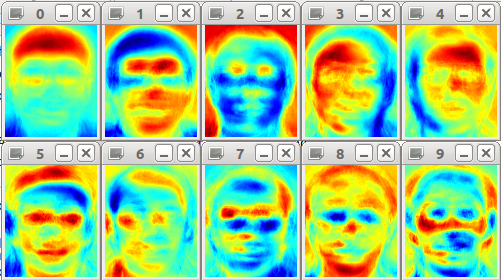
\includegraphics[scale=0.60]{img/libfacerec/eigenfaces_at.png}
\end{center}

So you see... learning the Eigenfaces is just as easy as writing:

\begin{lstlisting}[language=c++]
Eigenfaces model(images, labels);
\end{lstlisting}

and generating a prediction from the learned model is simply:

\begin{lstlisting}[language=c++]
int predicted = model.predict(testSample);
\end{lstlisting}

\subsubsection{Fisherfaces}

The following example shows how to calculate the Fisherfaces. I'll use the Yale Facedatabase A, just because the Fisherfaces look better.

\begin{lstlisting}[language=c++]
#include "opencv2/opencv.hpp"
#include "opencv2/highgui/highgui.hpp"

#include <iostream>
#include <fstream>
#include <sstream>

#include "facerec.hpp"

using namespace cv;
using namespace std;

void read_csv(const string& filename, vector<Mat>& images, vector<int>& labels, char separator = ';') {
    std::ifstream file(filename.c_str(), ifstream::in);
    if (!file)
        throw std::exception();
    string line, path, classlabel;
    while (getline(file, line)) {
        stringstream liness(line);
        getline(liness, path, separator);
        getline(liness, classlabel);
        images.push_back(imread(path,0));
        labels.push_back(atoi(classlabel.c_str()));
    }
}

int main(int argc, const char *argv[]) {
    // check for command line arguments
    if (argc != 2) {
        cout << "usage: " << argv[0] << " <csv.ext>" << endl;
        exit(1);
    }
    // path to your CSV
    string fn_csv = string(argv[1]);
    // images and corresponding labels
    vector<Mat> images;
    vector<int> labels;
    // read in the data
    try {
        read_csv(fn_csv, images, labels);
    } catch (exception& e) {
        cerr << "Error opening file \"" << fn_csv << "\"." << endl;
        exit(1);
    }
    // get width and height
    int width = images[0].cols;
    int height = images[0].rows;
    // get test instances
    Mat testSample = images[images.size() - 1];
    int testLabel = labels[labels.size() - 1];
    // ... and delete last element
    images.pop_back();
    labels.pop_back();
    // build the Fisherfaces model
    Fisherfaces model(images, labels);
    // test model
    int predicted = model.predict(testSample);
    cout << "predicted class = " << predicted << endl;
    cout << "actual class = " << testLabel << endl;
    // get the eigenvectors
    Mat W = model.eigenvectors();
    // show first 10 fisherfaces
    for (int i = 0; i < min(10, W.cols); i++) {
        // get eigenvector #i
        Mat ev = W.col(i).clone();
        // reshape to original site
        Mat grayscale = toGrayscale(ev.reshape(1, height));
        // show image (with Jet colormap)
        imshow(num2str(i), grayscale, colormap::Bone());
    }
    waitKey(0);
    return 0;
}
\end{lstlisting}

This yields the first 10 Fisherfaces (a Bone colormap coming with libfacerec was applied):

\begin{center}
	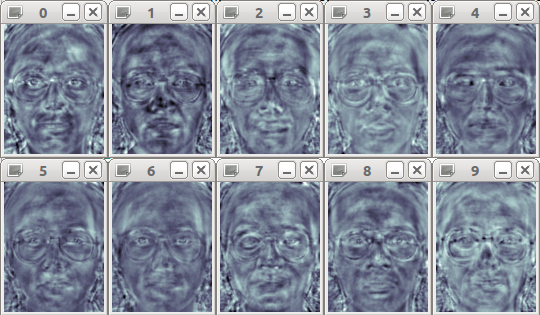
\includegraphics[scale=0.60]{img/libfacerec/fisherfaces_yale_a.png}
\end{center}

So you see... learning the Fisherfaces is just as easy as writing:

\begin{lstlisting}[language=c++]
Fisherfaces model(images, labels);
\end{lstlisting}

and generating a prediction from the learned model is simply:

\begin{lstlisting}[language=c++]
int predicted = model.predict(testSample);
\end{lstlisting}

\subsubsection{Saving and Loading a cv::FaceRecognizer}

Saving and loading a FaceRecognizer is very important, because training a FaceRecognizer can be a very time-intense task. Plus it’s often impossible to ship the whole face database to the user of your product, to learn the model. The task of saving and loading a FaceRecognizer is very easy with libfacerec. You only have to call \lstinline|cv::FaceRecognizer::load| for loading and \lstinline|cv::FaceRecognizer::save| for saving a FaceRecognizer.

In this example I'll show how to (1) learn the Eigenfaces of the AT\&T Facedatabase, (2) store the model to a YAML file, (3) load it again and (4) from the loaded model we’ll show the first 10 Eigenfaces.

\begin{lstlisting}[language=c++]
#include "opencv2/opencv.hpp"
#include "opencv2/highgui/highgui.hpp"

#include <iostream>
#include <fstream>
#include <sstream>

#include "facerec.hpp"

using namespace cv;
using namespace std;

void read_csv(const string& filename, vector<Mat>& images, vector<int>& labels, char separator = ';') {
    std::ifstream file(filename.c_str(), ifstream::in);
    if (!file)
        throw std::exception();
    string line, path, classlabel;
    while (getline(file, line)) {
        stringstream liness(line);
        getline(liness, path, separator);
        getline(liness, classlabel);
        images.push_back(imread(path,0));
        labels.push_back(atoi(classlabel.c_str()));
    }
}

int main(int argc, const char *argv[]) {
    // check for command line arguments
    if (argc != 2) {
        cout << "usage: " << argv[0] << " <csv.ext>" << endl;
        exit(1);
    }
    // path to your CSV
    string fn_csv = string(argv[1]);
    // images and corresponding labels
    vector<Mat> images;
    vector<int> labels;
    // read in the data
    try {
        read_csv(fn_csv, images, labels);
    } catch (exception& e) {
        cerr << "Error opening file \"" << fn_csv << "\"." << endl;
        exit(1);
    }
    // get width and height
    int width = images[0].cols;
    int height = images[0].rows;
    // get test instances
    Mat testSample = images[images.size() - 1];
    int testLabel = labels[labels.size() - 1];
    // ... and delete last element
    images.pop_back();
    labels.pop_back();
    // build the Fisherfaces model
    Eigenfaces model0(images, labels);
    // then save the model
    model0.save("eigenfaces_at.yml");
    // now load it from another object
    Eigenfaces model1;
    model1.load("eigenfaces_at.yml");
    // get the eigenvectors
    Mat W = model1.eigenvectors();
    // show first 10 fisherfaces
    for (int i = 0; i < min(10, W.cols); i++) {
        // get eigenvector #i
        Mat ev = W.col(i).clone();
        // reshape to original site
        Mat grayscale = toGrayscale(ev.reshape(1, height));
        // show image (with Jet colormap)
        imshow(num2str(i), grayscale, colormap::Jet());
    }
    waitKey(0);
    return 0;
}
\end{lstlisting}

\lstinline|eigenfaces_at.yml| was created on your filesystem and now contains the model state. We’ll simply show the first 10 lines with \lstinline|head eigenfaces_at.yml|:

\begin{lstlisting}
philipp@mango:~/github/libfacerec-build$ head eigenfaces_at.yml
%YAML:1.0
num_components: 399
mean: !!opencv-matrix
   rows: 1
   cols: 10304
   dt: d
   data: [ 8.5558897243107765e+01, 8.5511278195488714e+01,
       8.5854636591478695e+01, 8.5796992481203006e+01,
       8.5952380952380949e+01, 8.6162907268170414e+01,
       8.6082706766917283e+01, 8.5776942355889716e+01,
\end{lstlisting}

And here are the Eigenfaces from the stored model:

\begin{center}
	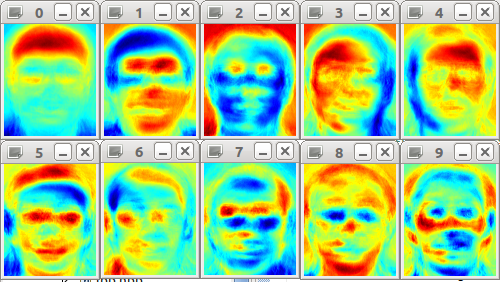
\includegraphics[scale=0.60]{img/libfacerec/stored_loaded_eigenfaces_at.png}
\end{center}

\subsubsection{Gender Classification}

A lot of people interested in face recognition are also interested in gender classification of faces. In this tutorial you’ll learn how to perform gender classification with OpenCV and libfacerec. First of all you’ll need some sample images of male and female faces. I have decided to search celebrity faces using Google Images with the faces filter turned on (my god, they have great algorithms at Google!).

My database has 8 male and 5 female subjects, each with 10 images. Here are the names if you aren’t that creative:

\begin{itemize}
 \item Angelina Jolie
 \item Arnold Schwarzenegger
 \item Brad Pitt
 \item Emma Watson
 \item George Clooney
 \item Jennifer Lopez
 \item Johnny Depp
 \item Justin Timberlake
 \item Katy Perry
 \item Keanu Reeves
 \item Naomi Watts
 \item Patrick Stewart
 \item Tom Cruise
\end{itemize}

All images were chosen to have a frontal face perspective, were aligned at the eyes and have been cropped to equal size, just like this set of George Clooney images:

\begin{center}
	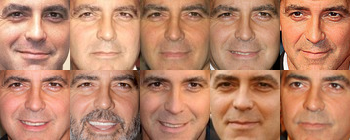
\includegraphics[scale=0.60]{img/libfacerec/gender_classification/clooney.png}
\end{center}

If we want to decide wether a person is male or female, we must use a class-specific method, in order to learn the discriminative features of both classes. The Eigenfaces method is based on a Principal Component Analysis, which is an unsupervised method, hence it is not suited for this task. The Fisherfaces method instead yields a class-specific linear projection, so it is better suited for the gender classification task. The Fisherfaces method actually performs very good. You can read my writeup on this at \href{http://www.bytefish.de/blog/gender_classification}.

In the code I will read the images from a CSV file gender.txt, which looks like this for my sample images:

\begin{lstlisting}
/home/philipp/facerec/data/gender/male/crop_keanu_reeves/keanu_reeves_01.jpg;0
/home/philipp/facerec/data/gender/male/crop_keanu_reeves/keanu_reeves_02.jpg;0
/home/philipp/facerec/data/gender/male/crop_keanu_reeves/keanu_reeves_03.jpg;0
...
/home/philipp/facerec/data/gender/female/crop_katy_perry/katy_perry_01.jpg;1
/home/philipp/facerec/data/gender/female/crop_katy_perry/katy_perry_02.jpg;1
/home/philipp/facerec/data/gender/female/crop_katy_perry/katy_perry_03.jpg;1
...
/home/philipp/facerec/data/gender/male/crop_brad_pitt/brad_pitt_01.jpg;0
/home/philipp/facerec/data/gender/male/crop_brad_pitt/brad_pitt_02.jpg;0
/home/philipp/facerec/data/gender/male/crop_brad_pitt/brad_pitt_03.jpg;0
...
/home/philipp/facerec/data/gender/female/crop_emma_watson/emma_watson_08.jpg;1
/home/philipp/facerec/data/gender/female/crop_emma_watson/emma_watson_02.jpg;1
/home/philipp/facerec/data/gender/female/crop_emma_watson/emma_watson_03.jpg;1
\end{lstlisting}

You see were this leads to? The label \lstinline|0| is for male subjects and label \lstinline|1| is for female subjects. The Fisherfaces code is the same as above:

\begin{lstlisting}[language=c++]
#include "opencv2/opencv.hpp"
#include "opencv2/highgui/highgui.hpp"

#include <iostream>
#include <fstream>
#include <sstream>

#include "facerec.hpp"

using namespace cv;
using namespace std;

void read_csv(const string& filename, vector<Mat>& images, vector<int>& labels, char separator = ';') {
    std::ifstream file(filename.c_str(), ifstream::in);
    if (!file)
        throw std::exception();
    string line, path, classlabel;
    while (getline(file, line)) {
        stringstream liness(line);
        getline(liness, path, separator);
        getline(liness, classlabel);
        images.push_back(imread(path,0));
        labels.push_back(atoi(classlabel.c_str()));
    }
}

int main(int argc, const char *argv[]) {
    // check for command line arguments
    if (argc != 2) {
        cout << "usage: " << argv[0] << " <csv.ext>" << endl;
        exit(1);
    }
    // path to your CSV
    string fn_csv = string(argv[1]);
    // images and corresponding labels
    vector<Mat> images;
    vector<int> labels;
    // read in the data
    try {
        read_csv(fn_csv, images, labels);
    } catch (exception& e) {
        cerr << "Error opening file \"" << fn_csv << "\"." << endl;
        exit(1);
    }
    // get width and height
    int width = images[0].cols;
    int height = images[0].rows;
    // get test instances
    Mat testSample = images[images.size() - 1];
    int testLabel = labels[labels.size() - 1];
    // ... and delete last element
    images.pop_back();
    labels.pop_back();
    // build the Fisherfaces model
    Fisherfaces model(images, labels);
    // test model
    int predicted = model.predict(testSample);
    cout << "predicted class = " << predicted << endl;
    cout << "actual class = " << testLabel << endl;
    // get the eigenvectors
    Mat W = model.eigenvectors();
    // show first 10 fisherfaces
    for (int i = 0; i < min(10, W.cols); i++) {
        // get eigenvector #i
        Mat ev = W.col(i).clone();
        // reshape to original site
        Mat grayscale = toGrayscale(ev.reshape(1, height));
        // show image (with Jet colormap)
        imshow(num2str(i), grayscale, colormap::Jet());
    }
    waitKey(0);
    return 0;
}
\end{lstlisting}

If you run the program with your gender.txt, you’ll see the Fisherface that best separates male and female images:

\begin{center}
	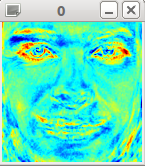
\includegraphics[scale=0.60]{img/libfacerec/gender_classification/fisherface_0.png}
\end{center}
